\section{Inlining blocks}

The blocks which have only one incoming block and are not blocks that appear after a recursive call can be inlined in
the incoming block. This is accomplished by marking the blocks that can be inlined first and then visiting the blocks
that cannot be inlined in order to generate the new blocks.

An example of this pass is provided in \labelindexref{Figure}{img:inline-blocks}. A second example is provided in
\labelindexref{Figure}{img:inline1}. This is the reduced control flow graph obtained from
\labelindexref{Figure}{img:trivial-after}.

\begin{figure}[htb]
    \begin{subfigure}[b]{.5\textwidth}
        \centering
        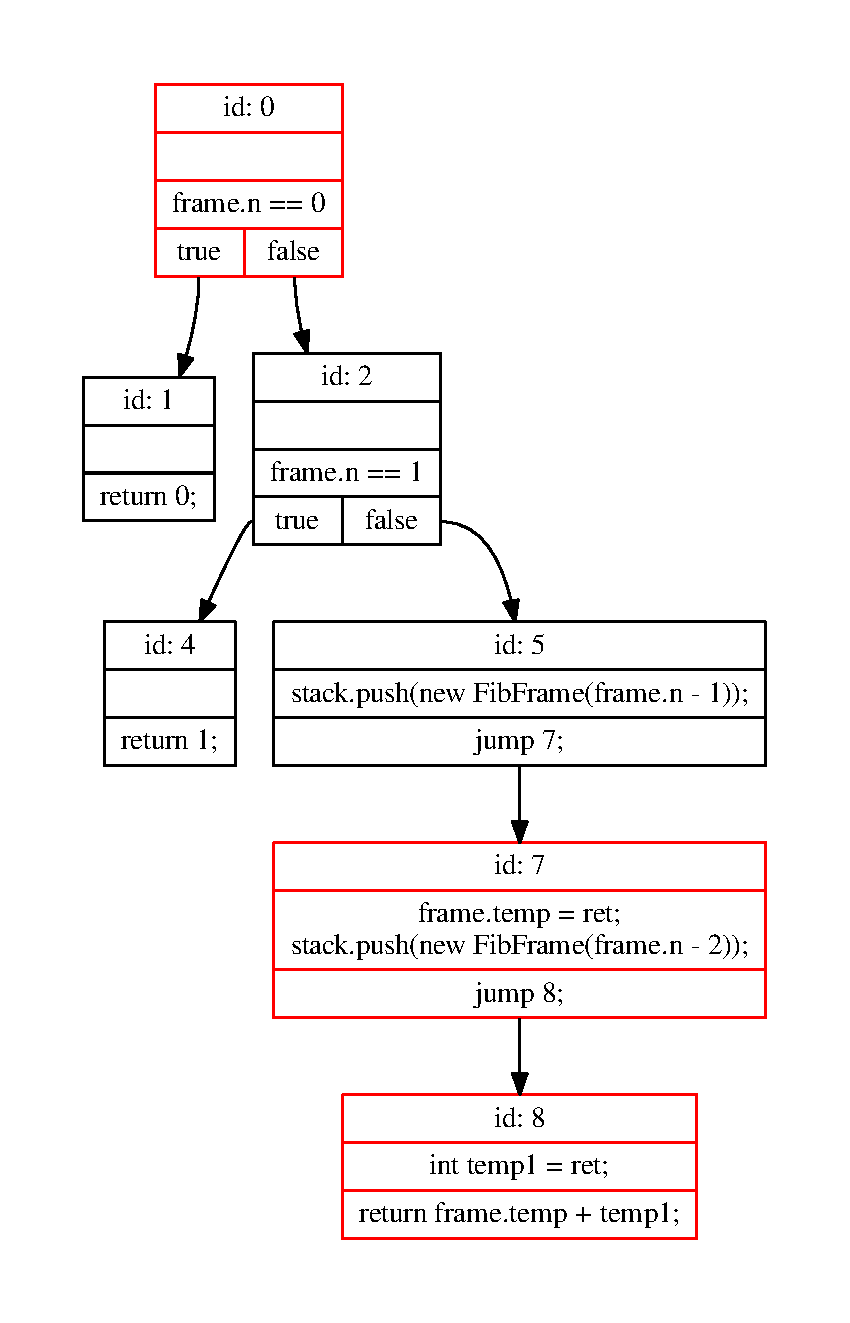
\includegraphics[height=3in]{src/graph/inline-before.pdf}
        \caption{Before}
    \end{subfigure}
    \begin{subfigure}[b]{.5\textwidth}
        \centering
        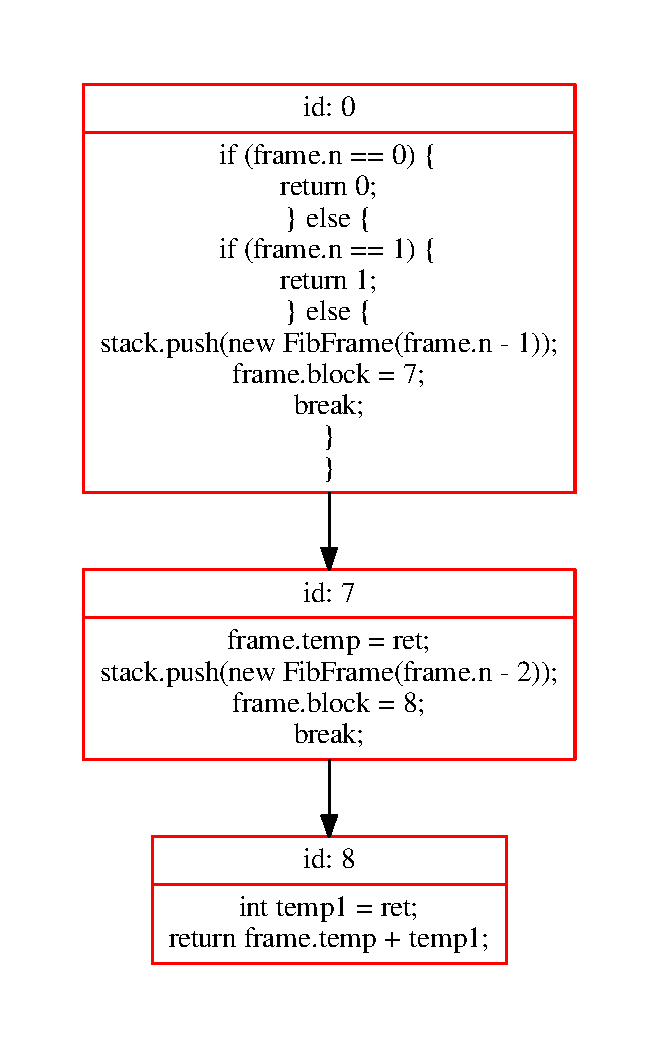
\includegraphics[height=3in]{src/graph/inline-after.pdf}
        \caption{After}
    \end{subfigure}
    \caption{Inlining blocks \label{img:inline-blocks}}
\end{figure}

\begin{figure}[htb]
    \centering
    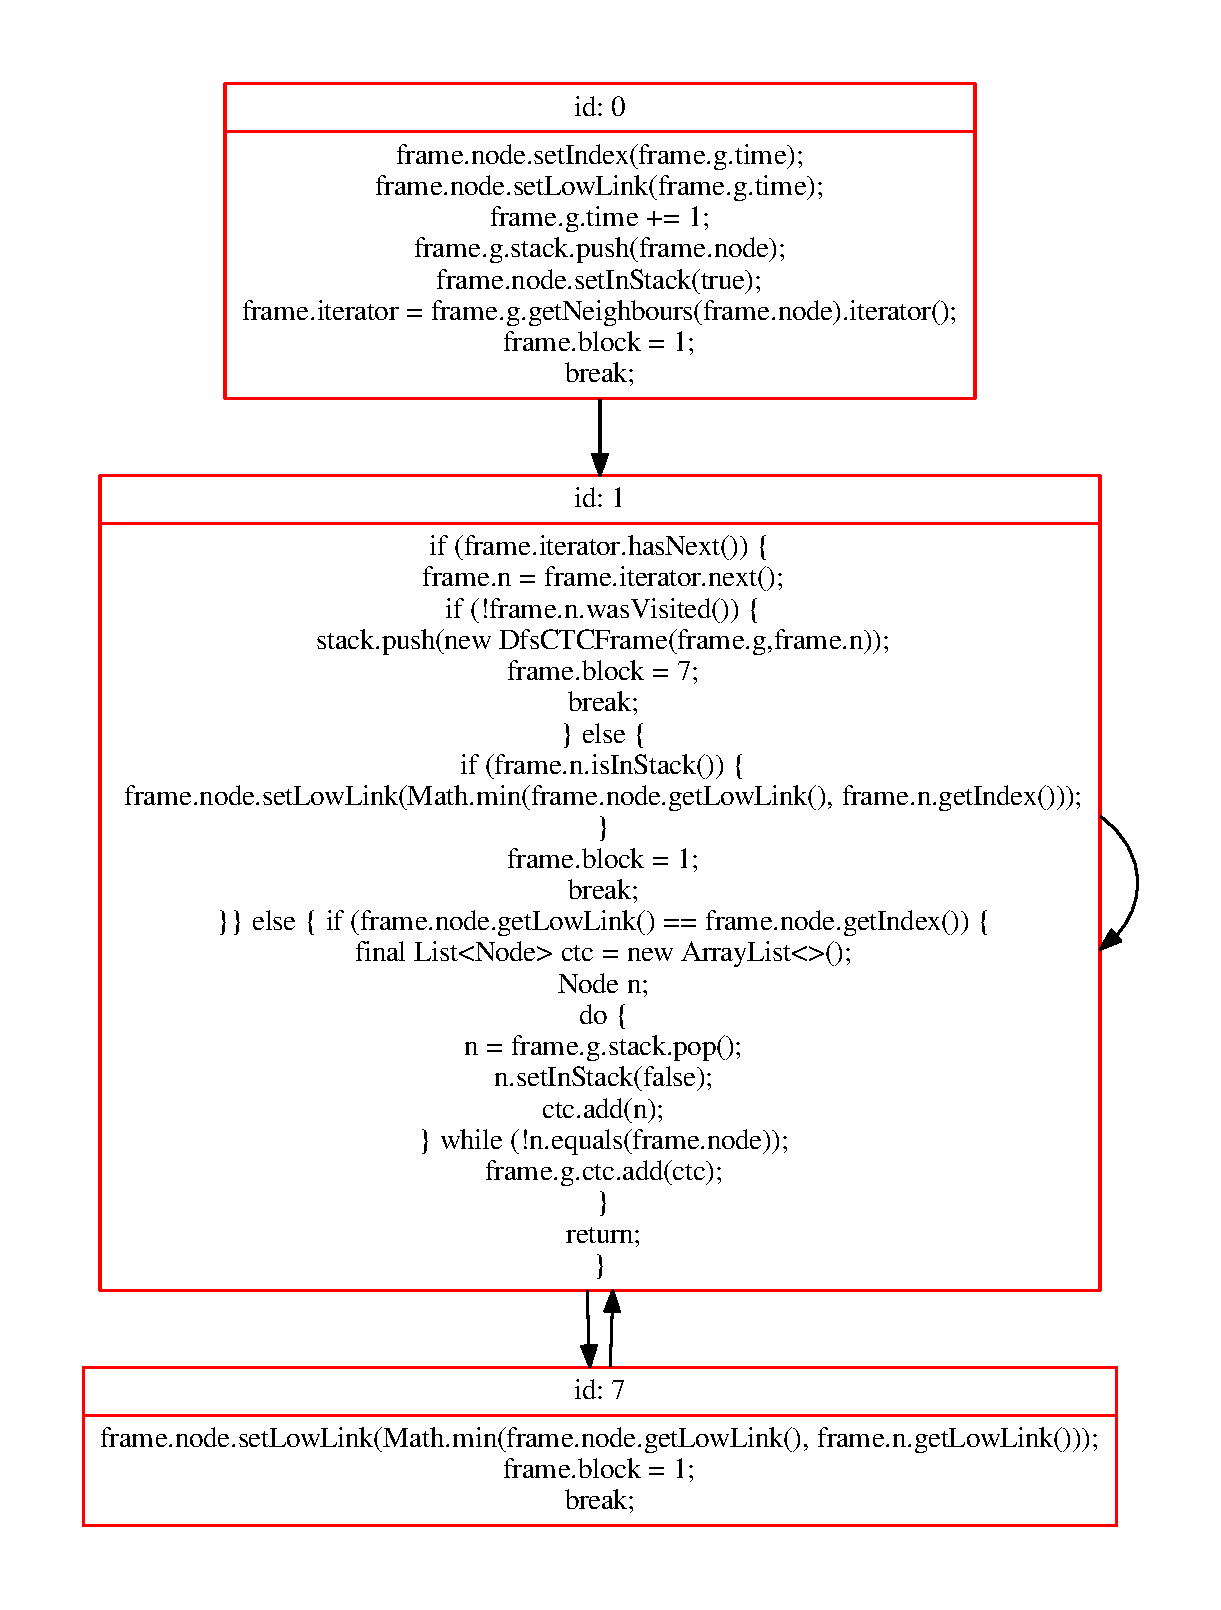
\includegraphics[width=.5\textwidth]{src/graph/inline-after-1.pdf}
    \caption{The reduced CFG\label{img:inline1}}
\end{figure}